\chapter{Appendix B}
\setcounter{figure}{0}
\renewcommand{\thefigure}{B.\arabic{figure}}

\begin{figure}
    \centering
    \includegraphics[width=\textwidth]{Appendix/Figures/B1_port.png}
    \caption[Time series plots of d\textsubscript{Nuc-Graph} of 0.25M, 0.50M and 0.75M simulations]{Time series plots of d\textsubscript{Nuc-Graph} of 0.25M, 0.50M and 0.75M simulations. All distances are presented in units of $\angstrom$.}
\end{figure}

\begin{figure}
    \centering
    \includegraphics[width=\textwidth]{Appendix/Figures/B2_port.png}
    \caption[Probability distribution of d\textsubscript{Nuc-Graph} of 0.25M, 0.50M and 0.75M simulations]{Probability distribution of d\textsubscript{Nuc-Graph} of 0.25M, 0.50M and 0.75M simulations. All distances are presented in units of $\angstrom$.}
\end{figure}

% \begin{figure}
%     \centering
%     \includegraphics[width=\textwidth]{Appendix/Figures/B3_port.png}
%     \caption[Time series plots for number of $\pi$-stacks and hydrogen - bonded dimers in 0.60M simulations]{Time series plots for number of (a) $\pi$-stacks and (b) hydrogen - bonded dimers in 0.60M simulations.}
% \end{figure}

\begin{figure}
    \centering
    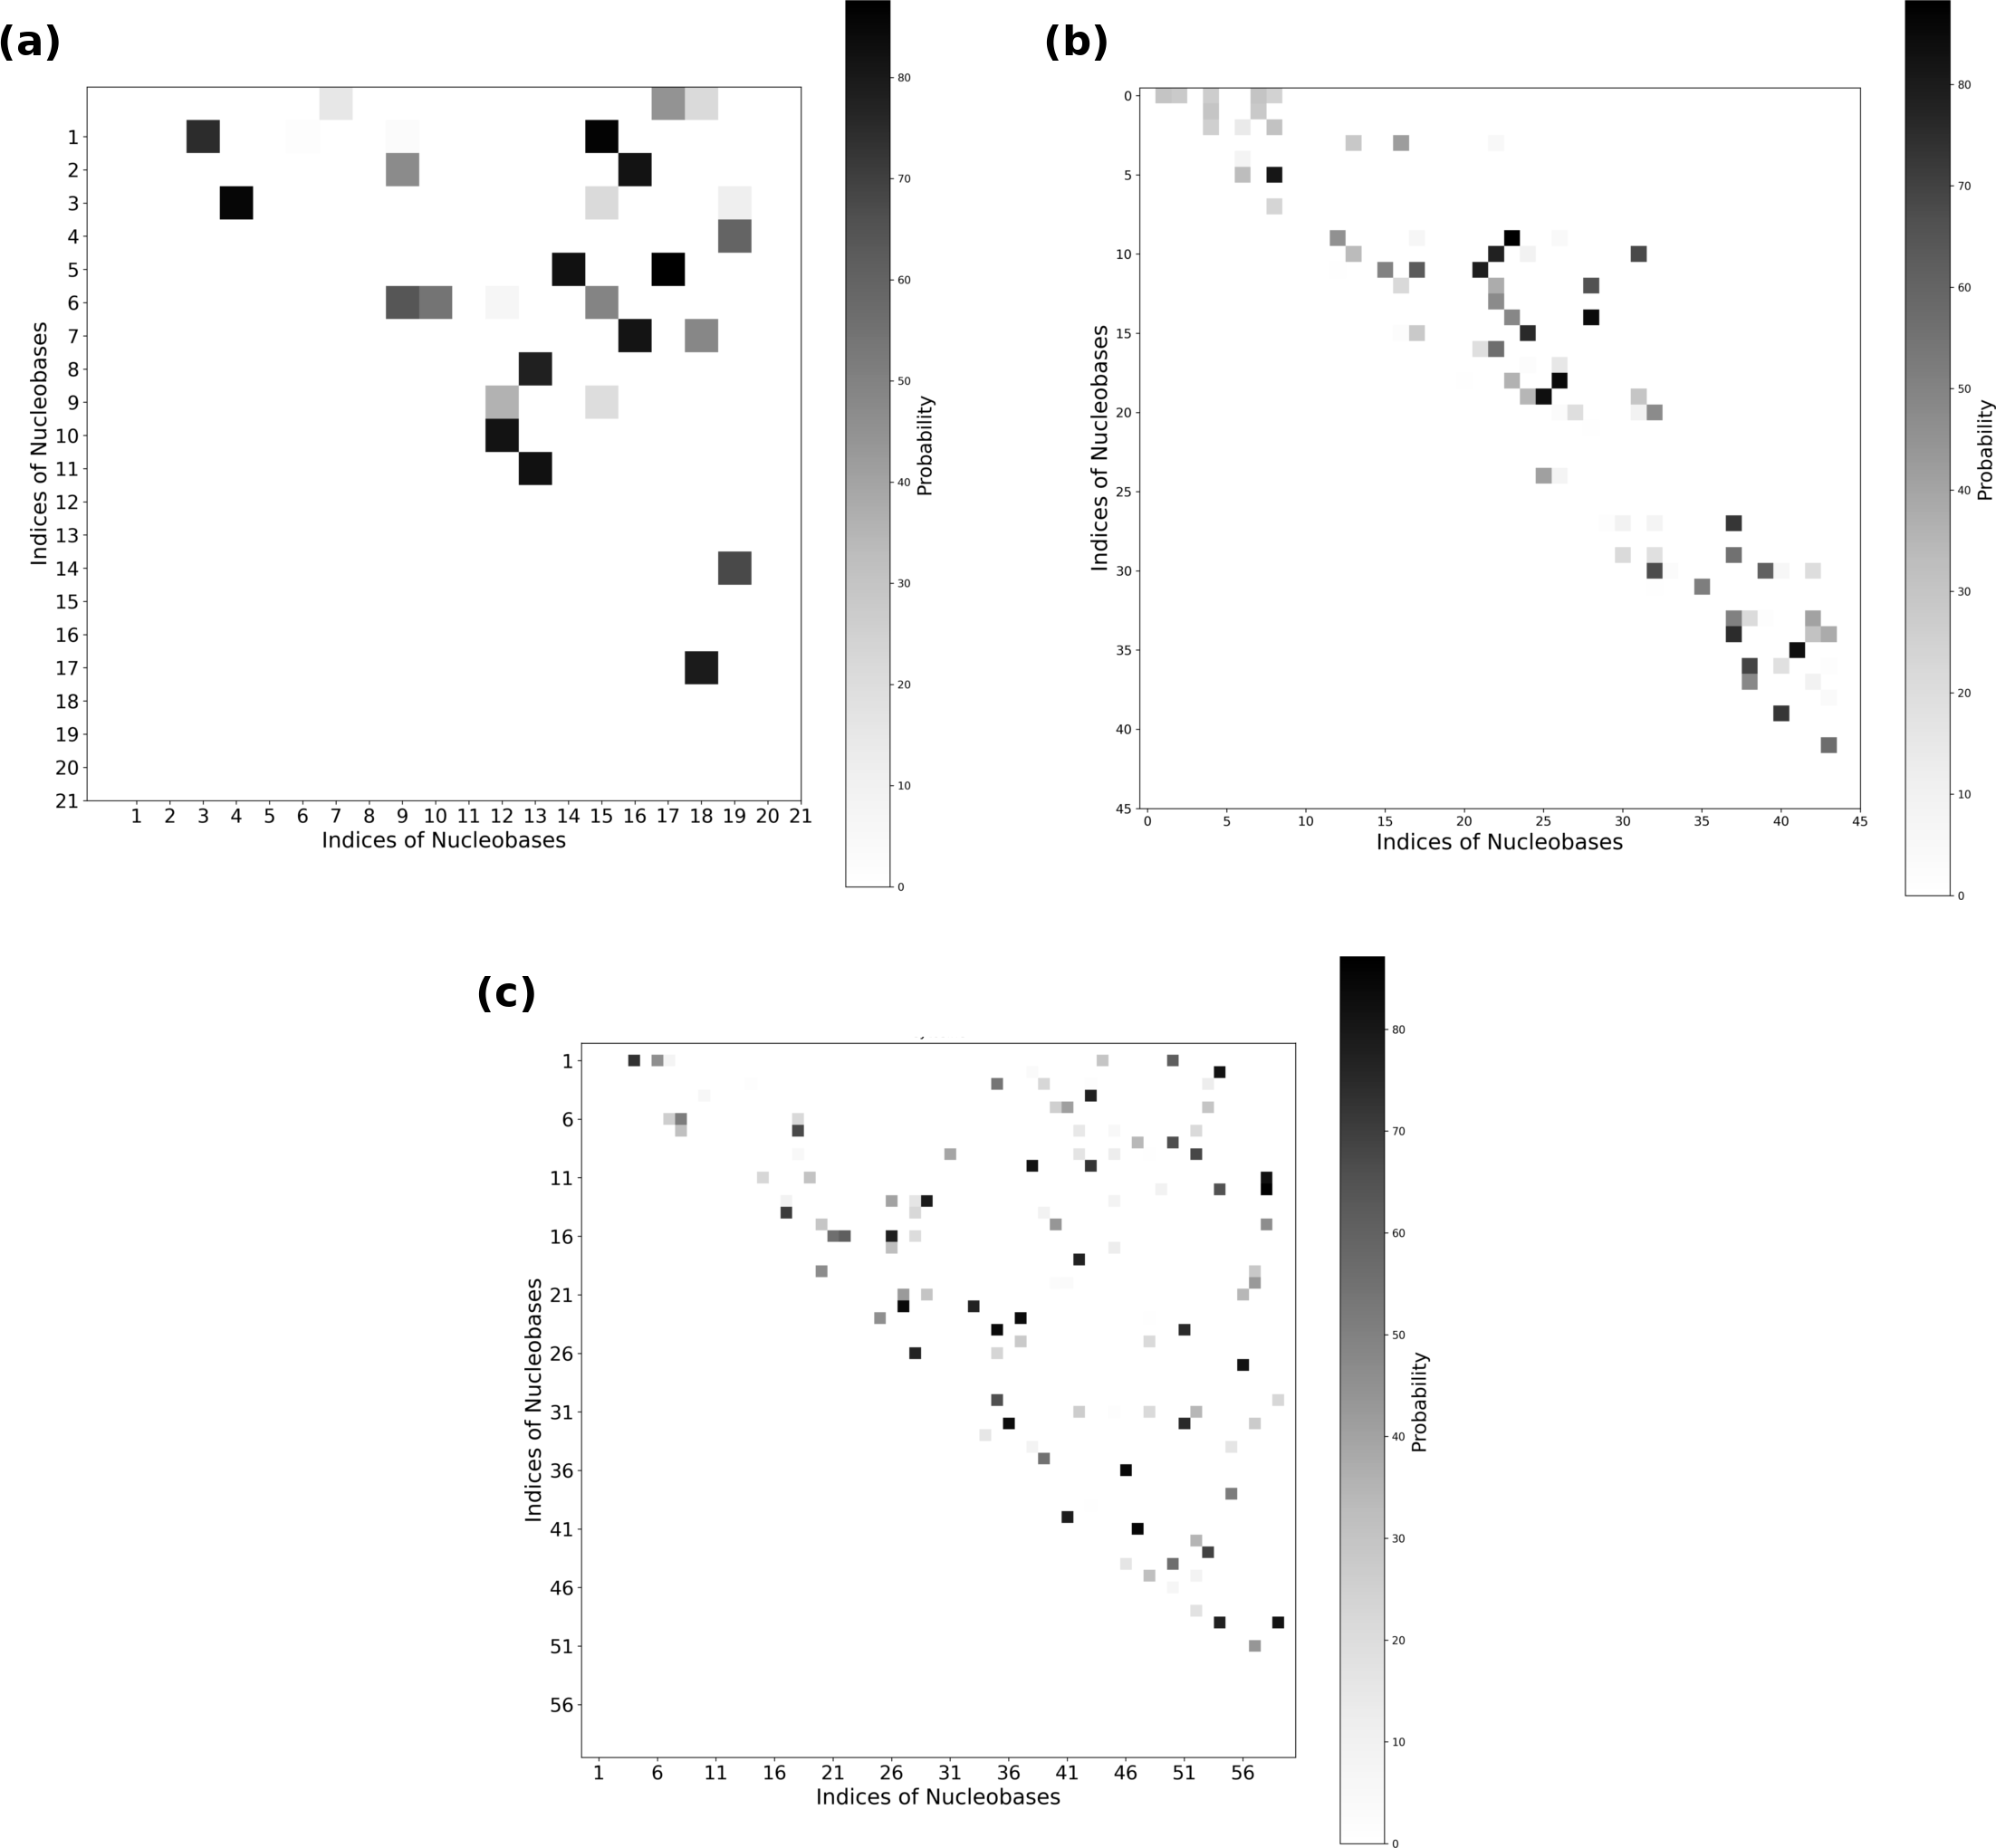
\includegraphics[width=\textwidth]{Appendix/Figures/B4_port.png}
    \caption[Heat map plots depicting the probabilities of different hydrogen - bonded dimers within the simulation box for 0.25M, 0.50M and 0.75M nucleobase - graphene simulations]{Heat map plots depicting the probabilities of different hydrogen - bonded dimers within the simulation box for (a) 0.25M, (b) 0.50M and (c) 0.75M nucleobase - graphene simulations. Probabilities are calculated as number of occurances of each dimer in the simulation trajectory.}
\end{figure}